% !TEX TS-program = pdflatex
% !TEX encoding = UTF-8 Unicode

% This is a simple template for a LaTeX document using the "article" class.
% See "book", "report", "letter" for other types of document.

\documentclass[11pt, titlepage]{article} % use larger type; default would be 10pt

\usepackage[utf8]{inputenc} % set input encoding (not needed with XeLaTeX)

%%% Examples of Article customizations
% These packages are optional, depending whether you want the features they provide.
% See the LaTeX Companion or other references for full information.

%%% PAGE DIMENSIONS
\usepackage{geometry} % to change the page dimensions
\geometry{a4paper} % or letterpaper (US) or a5paper or....
\geometry{margin=2cm, headsep=5mm, includefoot, includehead}

\usepackage{graphicx} % support the \includegraphics command and options
\graphicspath{{figures/}} % Location of the graphics files
% \usepackage[parfill]{parskip} % Activate to begin paragraphs with an empty line rather than an indent

%%% PACKAGES
\usepackage{booktabs} % for much better looking tables
\usepackage{array} % for better arrays (eg matrices) in maths
\usepackage{paralist} % very flexible & customisable lists (eg. enumerate/itemize, etc.)
\usepackage{verbatim} % adds environment for commenting out blocks of text & for better verbatim
\usepackage{subfig} % make it possible to include more than one captioned figure/table in a single float
% These packages are all incorporated in the memoir class to one degree or another...

%%% HEADERS & FOOTERS
\usepackage{fancyhdr} % This should be set AFTER setting up the page geometry
\pagestyle{fancy} % options: empty , plain , fancy
\fancyhead{}
%%% SECTION TITLE APPEARANCE
\usepackage{sectsty}
\allsectionsfont{\sffamily\mdseries\upshape} % (See the fntguide.pdf for font help)
% (This matches ConTeXt defaults)

%%% ToC (table of contents) APPEARANCE
\usepackage[nottoc,notlof,notlot]{tocbibind} % Put the bibliography in the ToC
\usepackage[titles,subfigure]{tocloft} % Alter the style of the Table of Contents
\renewcommand{\cftsecfont}{\rmfamily\mdseries\upshape}
\renewcommand{\cftsecpagefont}{\rmfamily\mdseries\upshape} % No bold!

\usepackage{lastpage}
\usepackage{rotating}
\usepackage{textcomp} %get the correct micro sec display
\usepackage{float}
%---------- Enable IEEEtran.bst configurations ------
\usepackage{IEEEtrantools}
%----------------------------------------------------

%%% END Article customizations

%%% The "real" document content comes below...

%%% Header %%%%%%%%%%%%%%%%%%%%%%%%%%%%%
\setlength{\headheight}{53pt}
\lhead{MF2063 Embedded Systems Design Project \\		 
       ESS-NW/ESS-CAR \\
       Leon Fernandez, leonfe@kth.se}
\rhead{Final Report \\
       Version 1 \\
       \thepage(\pageref{LastPage})}
\renewcommand{\headrulewidth}{1pt}
%%%%%%%%%%%%%%%%%%%%%%%%%%%%%%%%%%%%%%%%

%%% Footer %%%%%%%%%%%%%%%%%%%%%%%%%%%%%
%\cfoot{blablablabla}
%\renewcommand{\footrulewidth}{0.4pt}
%%%%%%%%%%%%%%%%%%%%%%%%%%%%%%%%%%%%%%%%
%\date{} % Activate to display a given date or no date (if empty),
         % otherwise the current date is printed 

\begin{document}
%\maketitle
\bstctlcite{BSTcontrol} % IEEEtran.bst controls enabled


%----------------------------------------------------------------------------------------
%	TITLE PAGE
%----------------------------------------------------------------------------------------

\begin{titlepage} % Suppresses displaying the page number on the title page and the subsequent page counts as page 1
	\newcommand{\HRule}{\rule{\linewidth}{0.5mm}} % Defines a new command for horizontal lines, change thickness here
	
	\center % Centre everything on the page
	
	%------------------------------------------------
	%	Headings
	%------------------------------------------------
	
	\begin{figure}
   		\centering
    	
\includegraphics[scale=1]{kthLogo.png}
	\end{figure}
	
	\textsc{\LARGE KTH Mechatronics Advanced Course}\\[1cm] % Main heading such as the name of your university/college
	
	\textsc{\Large MF2063, HT 2018}\\[0.5cm] % Major heading such as course name
	
	\textsc{\Large FINAL REPORT}\\[0.5cm] % Major heading as well
	
	%------------------------------------------------
	%	Title
	%------------------------------------------------
	
	\HRule\\[0.4cm]
	
	{\huge\bfseries ESS-NW/ESS-CAR}\\[0.4cm] % Title of your document
	
	\HRule\\[1.5cm]	
	
	%------------------------------------------------
	%	Author(s)
	%------------------------------------------------
	
	\begin{minipage}{0.4\textwidth}
		\begin{flushleft}
			\large
                        \textsc{Jonas Ekman}
			\\
			\textsc{Yini Gao}
                        \\
                        \textsc{Jacob Kimblad}
		\end{flushleft}
	\end{minipage}
	~
	\begin{minipage}{0.4\textwidth}
		\begin{flushright}
			\large
                        \textsc{Leon Fernandez}
			\\
			\textsc{Fredrik Hyyrynen}
                        \\
                        \textsc{Yifan Ruan}
		\end{flushright}
	\end{minipage}
	
	% If you don't want a supervisor, uncomment the two lines below
        % and comment the code above
	%{\large\textit{Author}}\\
	%John \textsc{Smith} % Your name
	\vskip 8cm
	\begin{figure}[H]
   		\centering
    	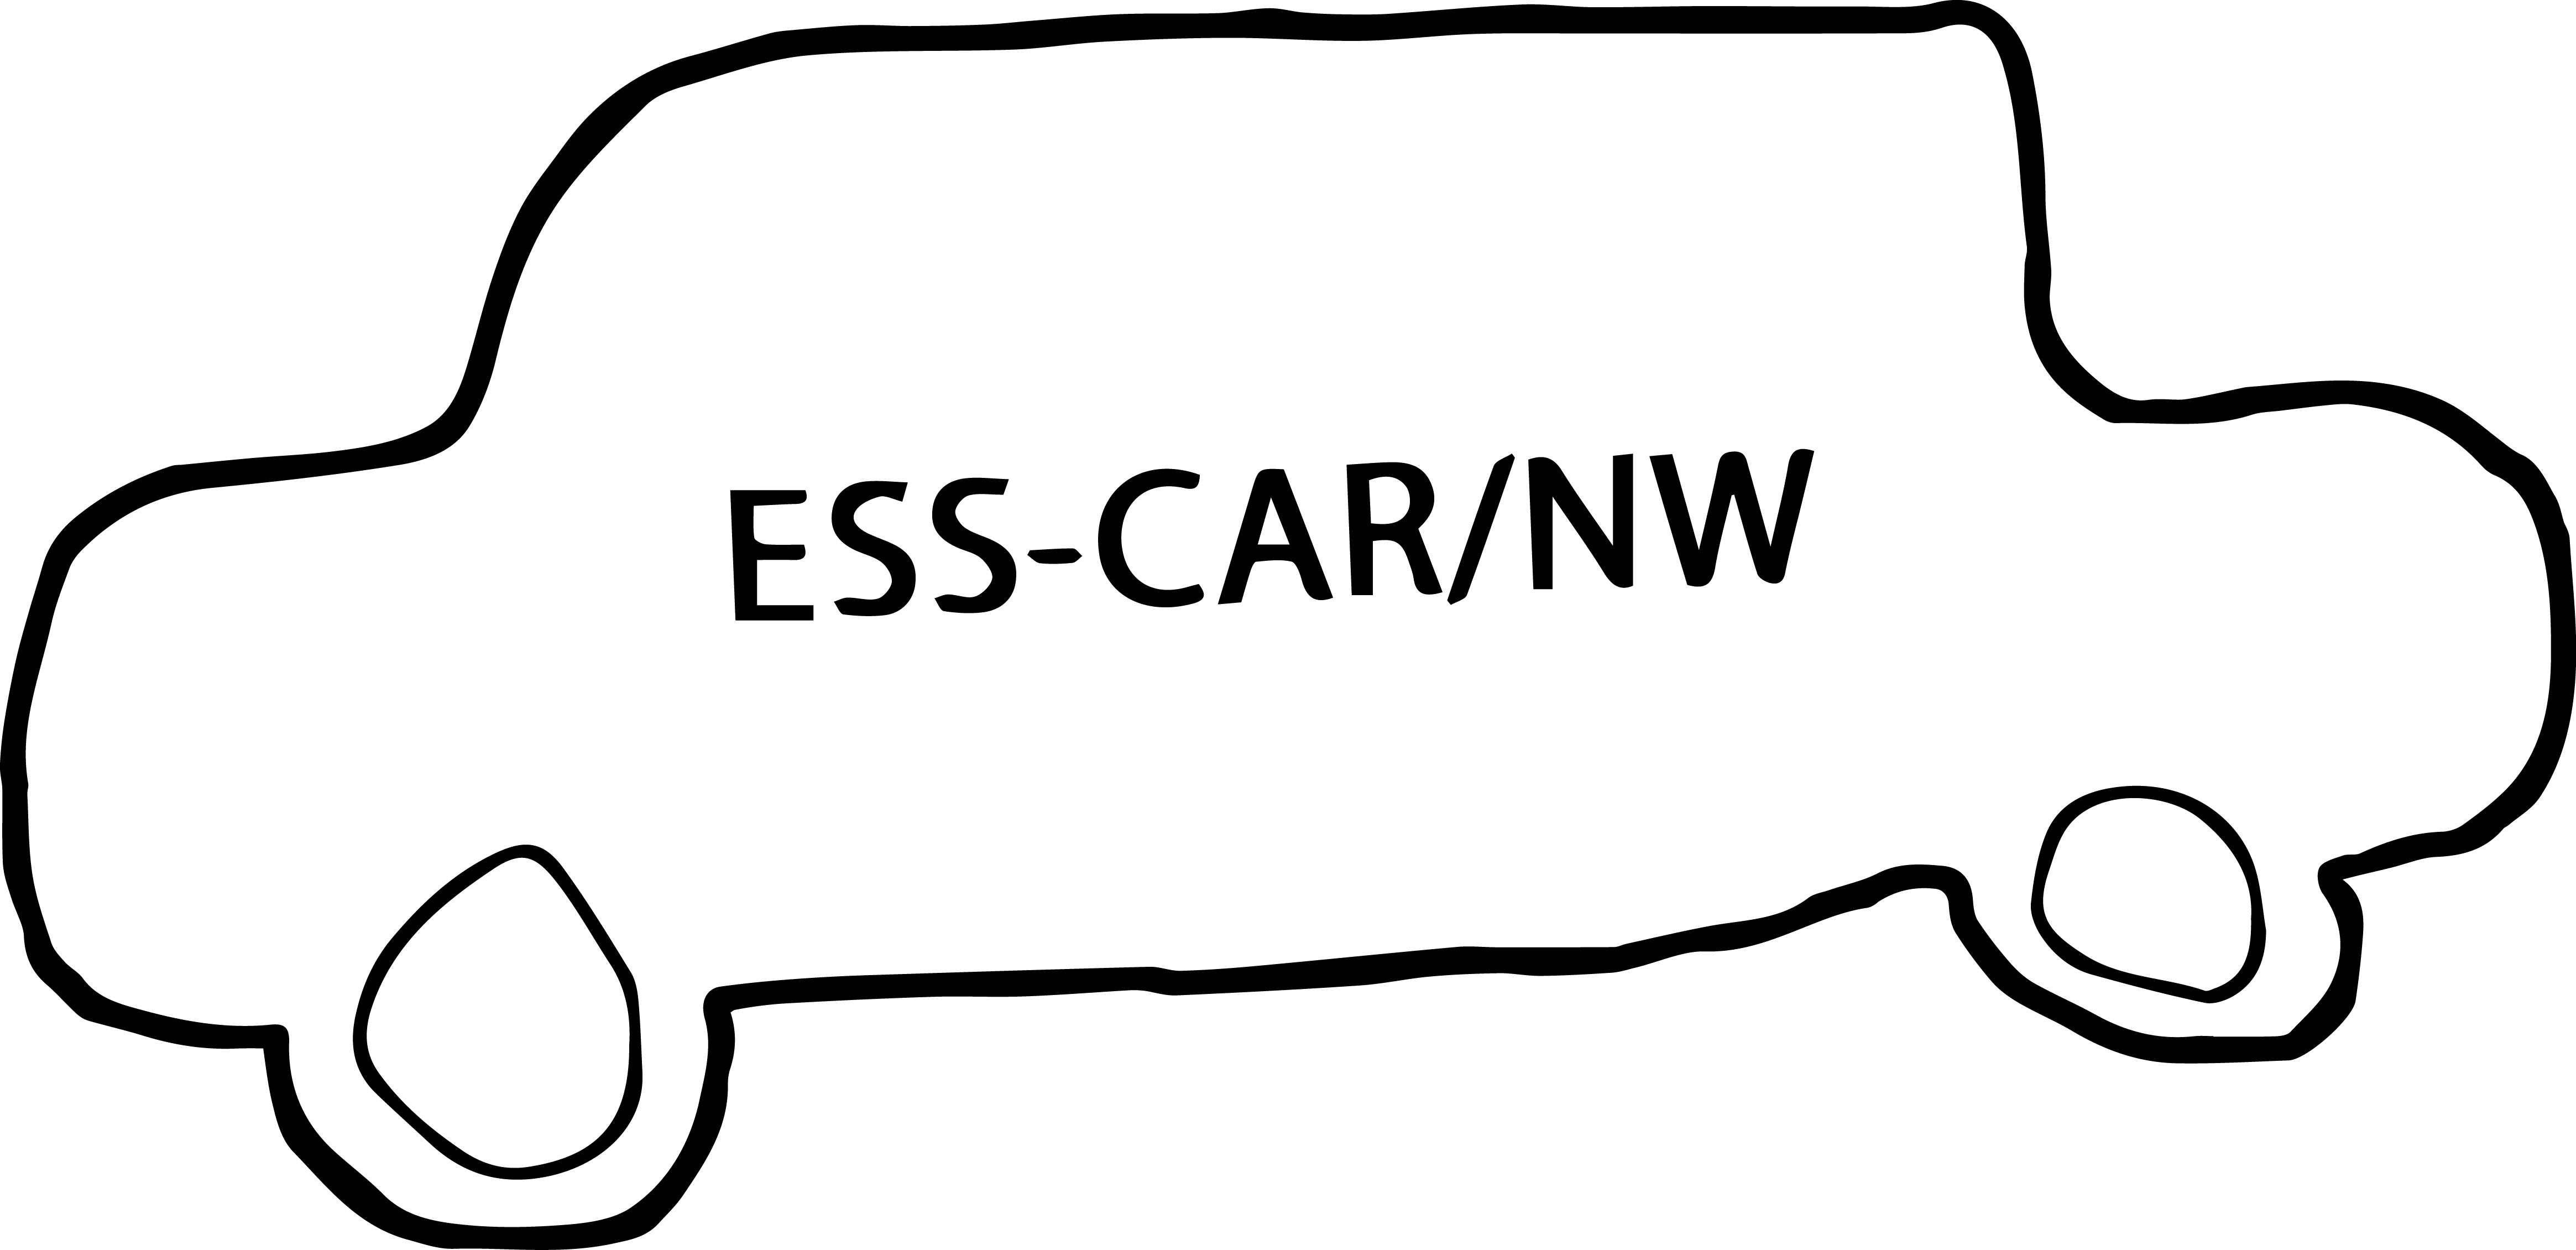
\includegraphics[scale=0.4]{funLogo.png}
	\end{figure}
	%------------------------------------------------
	%	Date
	%------------------------------------------------
	
	\vfill\vfill\vfill % Position the date 3/4 down the remaining page
	
	{\large\today} % Date, change the \today to a set date if you want
                       % to be precise
	
	%------------------------------------------------
	%	Logo
	%------------------------------------------------
	
	%\vfill\vfill
	%
\includegraphics[width=0.2\textwidth]{placeholder.jpg}\\[1cm]
        % Include a department/university logo
        % - this will require the graphicx package
	 
	%-------------------------------------------------------------------
	
	\vfill % Push the date up 1/4 of the remaining page
	
\end{titlepage}

%-------------------------------------------------------------------------

\clearpage
\section*{Abstract}
Abstract starts here,
what should be included:

The problem issue subject being addressed

How the problem is tackled

Overview of the results, and indication as to what level they solve the problem.

Implications of the results

%-------------------------------------------------------------------------
\clearpage
\tableofcontents

%-------------------------------------------------------------------------
\clearpage
\listoffigures

%-------------------------------------------------------------------------
\clearpage
\listoftables

%-------------------------------------------------------------------------
\clearpage
\section{Introduction}
This report presents the process and results of two projects "Embedded Service for Self-adaptive Network" (ESS-NW) and "Embedded Service for Self-adaptive Car" (ESS-CAR). This chapter will start by describing the background of the two projects. The next thing to be described is formulation, goals and motivation of the two projects. Following this will be a short discussion on the delimitations for our team. The last part of this chapter will present an explicit report disposition which helps readers to get a sense of the overall report.

\subsection{Background}

\subsubsection{Background subsection blabla}

\subsection{Project Description}

\subsubsection{Project Description sub blabla}

\subsection{Delimitations}

\subsection{Report disposition}

%-------------------------------------------------------------------------
\clearpage
\section{Literature Review and State of the Art}

\section{Network}
%-------------------------------------------------------------------------
\subsection{Software defined network}
Software-defined network (SDN) is a type of network where a controller decides how the traffic in the network should go. In a traditional network is the intelligence in the switches and they decided on what port the package should be sent out on. In SDN is a device called controller connected to all switches and monitors the traffic load on the links and find the most optimal path between node A to node B. The controller’s task is to request information from the switches about what links are up or down and the traffic load with this information and decides how packages should be forwarded on the switch. Because the controller can monitor the topology of the network is it easy to scale the network with new nodes and switches. 

Then the controller send directives to the switches uses it OpenFlow and it as a protocol used to send the forwarding plan to the switches.

sources !!!
%-------------------------------------------------------------------------
\subsection{Serial Peripheral Interface}
Serial Peripheral Interface (SPI) is a synchronous serial interface specification for short distance communication. SPI supports full duplex mode using a master-slave architecture with one single master, and the SPI master originates the whole communication. The SPI bus has four logic signals: serial clock (SCK), master output slave input (MOSI), master input and slave output (MISO), slave select (SS). The detailed pin mapping of SPI master and slaves is shown in figure ??.

% figure: one master and multiple slave connection
\begin{figure}[H]
	\centering
   	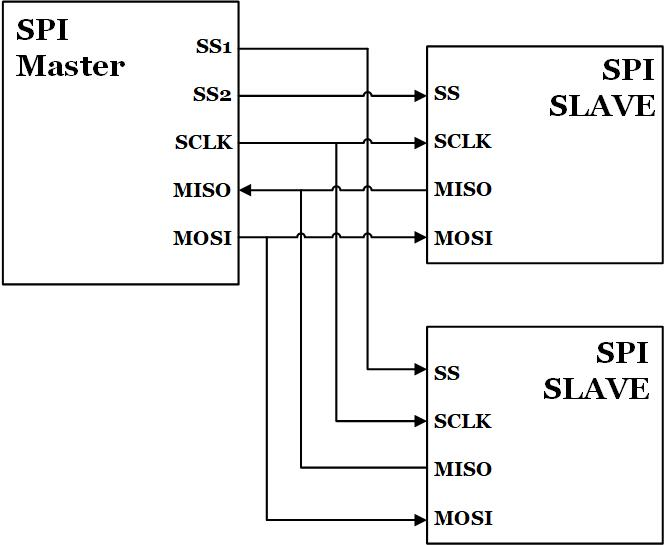
\includegraphics[scale=0.5]{spi-literature.jpg}
   	\caption{Connection of one SPI master and two SPI slaves}
    \label{fig:spi-literature}
\end{figure}

SPI has a higher throughput than those traditional transaction protocols, e.g. $I^{2}$C, UART, as it is not limited to any maximum clock speed enabling potentially high speed. And the hardware interface is pretty simple where slaves only use master's clock and are able to share the other three signals but the SS. Meanwhile, the software is not hard to implementation. For the opposite side, SPI has its limitations. There is no slave acknowledgement or hand-shaking mechanism in SPI, so the master could keep sending data to nowhere and not know it.


%-------------------------------------------------------------------------
\subsection{Assembly of the car}
 To make the car moving all the devices and components on the car has to placed on the car and because there many devices on the car that communicates via SDN and has all of them be placed in a efficient way. To do that needs some kind of platform be created to mount all the devices on and they are close to the other devices its depended on. 

%-------------------------------------------------------------------------

\subsection{Power Supply}
The car uses a 2 cell lithium battery what delivers a voltage of 7.2V. On the car is two different voltage level used, the first one is at 9V for a switch, and the second level is at 5V to power all the other components. 

To generate a voltage at 9V from 5V or 7.2V has some kind of DC-DC converter be build to generate a higher voltage. A DC-DC converter works as ...  



%-------------------------------------------------------------------------
\clearpage
\section{Methodology}
%%%%%%%%%%%%%%%%%%%%%%%%%%%%%%%%%%%%%%%%%%%%%%%%%%
%TODO chapter overview
%-------------------------------------------------------------------------
\subsection{Network}
%-------------------------------------------------------------------------
\subsubsection{Software defined network}

The SDN switches used in this implementation is the Zodiac FX from Northbound Networks. They are switches made for to support OpenFlow protocol and is designed to use in SDN networks. On the switch is 4 ports there one port has to be connected to the controller, all the other ports can be used to connect devices on. As shown in figure ?? is 5 devices connected to the network and the switches has to be connected to each other has the network 3 switches. 

Mininet is a Python-based application what an SDN network topology can be created and simulated to test that the controller works and analyse how the network will operate. The program also has the opportunity to connect the simulated topology to your physical SDN controller. 

The car network topology was simulated in Mininet to analyse its behaviour, and to develop code for the controller. Under this test did we discover what that Mininet simulation had a much lower delay then the real implementation had, even then the extra setings on the links and nodes was added. This resulted that Mininet could not be used to analyse the best topology for the car. It was instead used to simulate the network to create a code for the Ryu controller. 

%-------------------------------------------------------------------------
\subsection{VSOME/IP}
%-------------------------------------------------------------------------
\subsection{Engineering approaches ?}
\subsection{Tool-chains ?}
\subsection{Project management}
Scrum project management is used during the process of our projects.
%-------------------------------------------------------------------------
\subsection{Assembly of the car}

The car platform used in this project is a car platform is Turnigy SCT 2WD 1/10 Brushless Short Course Truck (KIT) upgraded version and it was provided by the stakeholders at the start of the project. 

To place all the required components on the car had some kind of platform be created to mount everything on. The requirements for the platform is if passible the car chassis should be able to fit on top of the car, all the device should be mounted on it and it should be easy to remove from the car. 

To make this platform was it first draw in a Cad Fusion 360 to make a 3D model of the car. This model could then be used to add models of the devices used in the car to find the optimal place for them, so the are places in at an easy position to get access too and close to its devices its depended on. The result of the design is shown in figure ??

%-------------------------------------------------------------------------
\subsection{Power Supply and PCB}

The power supply for the devices on the car is done via two different levels one at 5V and the second one at 9V. This requires some converter to converts the 7.2V from the battery to 5V and 9v. The 5V DC-DC converter is a module used in RC cars to ... 

The second converter is to generate the 9V and this is done via DC-DC converter called boost converter. The boost converter is in this design is ... 

The powering of all the devices will be done via USB-A connectors on the power support unit to get a modularity if a device and to be changed for a new type. All this USB-A connectors gives only an output of 5V. The powering of the external switch will be done via a cable mounted on the power unit and connected to the switch.
 

To mount all the USB connectors and the boost converter was a PCB designed to be able to have everything on one board. A PCB designed was made in Eagle to make the schematic and the layout. The layout of the board is shown in figure ?? 


To power the Arduinos was a specific PCB boards designed so they could easily be connected to a SPI interface. The layout of the boards is shown in figures ?? 


%-------------------------------------------------------------------------

\clearpage
\section{Implementation}

%-------------------------------------------------------------------------
\subsection{System overview}
maybe put communication diagram here

%-------------------------------------------------------------------------
\subsection{SDN network Implementation}

In the beginning of the project was floodlight that SDN controller framework we decided to work with. Under the project way was a lot of problem coming up to integrate floodlight on raspberry pi due to some java packages used in Floodlight was not supported, and it had difficulties to communicate with the SDN switches. This resulted in that another SDN framework was selected, and it was a framework called Ryu. Ryu was selected because it was well documented with some example code to start with, and it was developed in python, so it should be no problem with integrating it on a raspberry pi. 

\subsection{shared memory things}

\subsection{Communication between Beaglebone and Arduino ?}
%%%%%%%%%%%%%%%%%%%%%%%%%%%%%%%%%%%%%%
% SPI introduction in literature review, pros over UART
%TODO reference to the simple gpio library (github page)
% NOT SURE: PUT simple gpio lib to management chapter
%%%%%%%%%%%%%%%%%%%%%%%%%%%%%%%%%%%%%
As the Beaglebone only supports to be the master in a SPI connection, so we have two beaglebones with SPI configurations and each of them has two Arduino slaves. One Beaglebone has two spi devices: SPIDEV0 and SPIDEV1, and the SPIDEV1 device is disabled initially but is used for HDMI interface. 

In order to have one SPI device on Beaglebone connecting to multiple Arduino slaves, we use a third party C++ library called SimpleGPIO which enables us to use other general purpose pins as slave select of the SPI connection. Before we start communication with a specific Arduino slave, the corresponding slave select will be set to low, then we get access to that Arduino slave.

In the Arduino side, the communication request from the Beaglebone is treated as an interrupt. Then the Arduino writes/reads to/from the Serial Peripheral Data Register (SPDR). 
\subsection{Sensors}
Three categories of sensors are implemented in the prototype vehicle to monitor its surrounding environments. Data from distance sensors and speed sensor will be sent to an Arduino initially, then sent to corresponding Beaglebone. Data from Pi Camera will be sent to the Raspberry Pi which is directly connected to the main network.
%-------------------------------------------------------------------------
\subsubsection{Ultrasonic sensor}
%%%%%%%%%%%%%%%%%%%%%%%%%%%%%%%%%%%%%%%%%%%%%%%%%%%%%%%%%%%%%%
% put why we choose HC-SR04 in other chapter, e.g. methdology
%%%%%%%%%%%%%%%%%%%%%%%%%%%%%%%%%%%%%%%%%%%%%%%%%%%%%%%%%%%%%%
To get data from HC-SR04, a short 10\textmu s pulse should be supplied to the trig pin of ultrasonic sensor, then the sensor will send out an 8 cycle burst of ultrasound at 40 kHz and raise echo. The echo signal we get is a distance object which is pulse width and the range of the signal is in proportion. 

An Arduino Micro handles both the generating the trig pulse and interpreting the echo signal. The Arduino will set the output pin to low, wait for 5ms, set the pin to high, wait for 10ms, set the pin back to low. This is the process of generating the trig pulse. After the Arduino sends out the trig pulse, it waits for 2 ms, then reads the value from the pin connected to sensor's echo pin. The last step is convert the received value to distance in unit of centimeter.

%TODO distance sensor working process figure

\subsubsection{Reflective object sensor}
\subsubsection{Pi Camera}
In computer vision part, we tried to compare the performance of two different methods, which are object detection based on neural network and color detection using OpenCV.

The technique of transfer learning is used to apply MobileNet on RPI, which is an efficient model for mobile and embedded vision applications. The speed remains slow although hardware acceleration and multiprocessing have been carried out to improve.

By using OpenCV’s DNN module, we are able to pass input images through the deep neural network and get a output image with bounding box of specific object and label.

Since we are working on source constrained device Raspberry Pi, we need to make the network simple and decrease the computational cost, so we combined MobileNet with Single Shot Detector.

In order to optimize the Raspberry efficiently and use sufficiently limited resource and memory on it when running neural network, we firstly apply hardware optimization which is to install optimized OpenCV complie. So, ARM NEON as an optimization architecture extension for ARM processors is used. It is used for faster video stream processing, image analysis and speech recognition that is exactly what we are look for in our application. This architecture can execute multiple processing in the pipeline by a single instruction. Besides, VFPV3 as a floating point optimization is also used. After the first stage improvement, we get a 30 percent speed increase since we have make full use of the 4× ARM Cortex-A53, 

When it comes to second stage of optimization, multiprocessing is used to increase the speed of processing video stream. The I/O tasks, dislike CPU bound operations, always take lots of time and delay the process. So moving the reading of frames to a separate thread from frame processing can obtain higher speed. Otherwise, every time I/O port access Pi camera, the main thread of script is blocked until the frame is captured and return to script. Multiprocessing can decrease the influence of I/O on CPU heavy application like video stream processing, especially in our real-time case. Now we can obtain a detection result within 1 second.

Additionally, there is a trade off between accuracy and output speed. In our application, we set a threshold for the output, in more details, only when the confidence score of detection result is high enough (above the specified threshold), the result can be output as a signal to steer the car. Otherwise, it will grab another frame and do the object detection for the other iteration. As a result, if the threshold confidence score of output increase, the output speed will decrease.

Since the object detection method outputs result slowly, we move on to the other method which is color detection using OpenCV to see whether the  speed is fast enough to be applied on a car prototype.

We define the upper and lower limits for pixel values to classify three colors. Then specify which pixels fall into specified upper and lower range by masking. The speed of color detection is fast and also accurate enough for real-time application.

So we finally apply the color detection on our car, we use the result of detection to steer the car.



\subsection{Controlling actuators}
%-------------------------------------------------------------------------
\subsubsection{Steering servo}
%-------------------------------------------------------------------------
\subsubsection{Motor ESC}
%-------------------------------------------------------------------------

\subsection{Assembly of the car}


%-------------------------------------------------------------------------
\subsection{Power Supply and PCB}

The idea of was to order the PCBs from a company, but due to course regulation ware we not alowed to order PCBs from China, and companies in Europe were to expensive to order from. This resulted in what we could not implemented the boost converter we hade design due to the milling machine in both prototype centre and in Mentorspace was broken and they could not mill the layout for the boost converter. Because the milling machines was broken could the PCB for the Arduinos also not be made. The only way we could continue with was to make the design on a prototyping board. 

The implementation is as shown in figure ?? 


%-------------------------------------------------------------------------


\clearpage
\section{Verification and Validation}

%-------------------------------------------------------------------------
\clearpage
\section{Results}

%-------------------------------------------------------------------------
\clearpage
\section{Discussion and Conclusion}

%-------------------------------------------------------------------------
\clearpage
\section{Future Work}
%-------------------------------------------------------------------------
\clearpage
%TODO reference
\clearpage
%-------------------------------------------------------------------------
\clearpage
%TODO appendix
\appendix
\clearpage

\end{document}
